\documentclass[../main.tex]{subfiles}
\begin{document}
    \chapter{Evaluation}\label{ch:evaluation}
    
	In this chapter we evaluate the steps we took in this research.
	We first describe the setup of the experiment in section \ref{sec:evaluation_experiment_setup}.
	Next we present the results in section \ref{sec:evaluation_results}.
	In section \ref{sec:evaluation_analysis} we analyse the measured results.
	
	% Methode: Hoe zet je het experiment op en wat ga je meten
	\section{Experiment setup}\label{sec:evaluation_experiment_setup}
	
	In order to validate the this research we have tested the type inference on a selection of the 30 most popular packages of Packagist\footnotemark.
	\footnotetext{https://packagist.org/explore/popular, July 2014}
	Packagist is a repository for Composer\footnotemark projects.
	\footnotetext{https://getcomposer.org/, July 2014}
	Composer is a dependency manager for PHP.
	All projects have between 2 and 6 million downloads, so they should be representative for our research because they are frequently used in live applications.
	The selection of projects, sorted on total lines of code, is listed in table \ref{table:corpus}.
	Due to performance reasons we are only able to analyse the smaller projects.
	The statistics are generated using phploc\footnotemark.
	\footnotetext{https://github.com/sebastianbergmann/phploc, July 2014}

	
\npaddmissingzero
\npfourdigitsep
\begin{table}[H]
  \centering
  \scriptsize
  \begin{tabular}{@{}lllrrrrrrrr@{}} \toprule
     \multicolumn{3}{c}{Product}        & \multicolumn{2}{c}{Files} & \multicolumn{3}{c}{Objects}        & \multicolumn{3}{c}{Lines of code} \\
     \cmidrule(l{2pt}r{2pt}){1-3}       \cmidrule(l{2pt}r{2pt}){4-5} \cmidrule(l{2pt}r{2pt}){6-8}        \cmidrule(l{2pt}r{2pt}){9-11}                    
     Vendor & Project* & Version           & D$^1$         & F$^2$          & C$^3$ & I$^4$ & T$^5$ & Total $\uparrow$ & \multicolumn{2}{c}{Logical} \\ \midrule
doctrine & lexer & v1.0 & 2 & 7 & \numprint{3} & \numprint{0} & \numprint{0} & \numprint{733} & \numprint{128} & (17.46\%) \\
phpunit & php-timer & 1.0.5 & 5 & 11 & \numprint{5} & \numprint{0} & \numprint{0} & \numprint{740} & \numprint{117} & (15.81\%) \\
phpunit & php-text-template & 1.2.2 & 5 & 11 & \numprint{5} & \numprint{0} & \numprint{0} & \numprint{768} & \numprint{125} & (16.28\%) \\
doctrine & inflector & v1.0 & 2 & 7 & \numprint{3} & \numprint{0} & \numprint{0} & \numprint{853} & \numprint{130} & (15.24\%) \\
psr-fig & log & 1.0.0 & 3 & 15 & \numprint{8} & \numprint{2} & \numprint{2} & \numprint{1039} & \numprint{155} & (14.92\%) \\
phpunit & php-file-iterator & 1.3.4 & 5 & 13 & \numprint{7} & \numprint{0} & \numprint{0} & \numprint{1071} & \numprint{176} & (16.43\%) \\
%symfony & filesystem & v2.5.3 & 3 & 11 & \numprint{5} & \numprint{2} & \numprint{0} & \numprint{1090} & \numprint{193} & (17.71\%) & \numprint{19} & (9.84\%) \\
%symfony & yaml & v2.5.3 & 3 & 16 & \numprint{11} & \numprint{1} & \numprint{0} & \numprint{2270} & \numprint{509} & (22.42\%) & \numprint{28} & (5.50\%) \\
%phpunit & php-token-stream & 1.2.2 & 6 & 13 & \numprint{169} & \numprint{0} & \numprint{0} & \numprint{2360} & \numprint{377} & (15.97\%) & \numprint{15} & (3.98\%) \\
%doctrine & collections & v1.2 & 3 & 18 & \numprint{11} & \numprint{3} & \numprint{0} & \numprint{2504} & \numprint{394} & (15.73\%) & \numprint{33} & (8.38\%) \\
%symfony & process & v2.5.3 & 3 & 19 & \numprint{14} & \numprint{1} & \numprint{0} & \numprint{3198} & \numprint{604} & (18.89\%) & \numprint{37} & (6.13\%) \\
%symfony & finder & v2.5.3 & 8 & 43 & \numprint{36} & \numprint{3} & \numprint{0} & \numprint{4976} & \numprint{909} & (18.27\%) & \numprint{80} & (8.80\%) \\
%symfony & dom-crawler & v2.5.3 & 12 & 63 & \numprint{53} & \numprint{6} & \numprint{0} & \numprint{7825} & \numprint{1296} & (16.56\%) & \numprint{157} & (12.11\%) \\
%symfony & translation & v2.5.3 & 21 & 121 & \numprint{97} & \numprint{20} & \numprint{0} & \numprint{12345} & \numprint{2299} & (18.62\%) & \numprint{257} & (11.18\%) \\
%symfony & console & v2.5.3 & 17 & 84 & \numprint{66} & \numprint{13} & \numprint{2} & \numprint{13546} & \numprint{2556} & (18.87\%) & \numprint{246} & (9.62\%) \\
%symfony & http-foundation & v2.5.3 & 16 & 90 & \numprint{76} & \numprint{10} & \numprint{0} & \numprint{14179} & \numprint{2262} & (15.95\%) & \numprint{154} & (6.81\%) \\
%twig & twig & v1.16.0 & 18 & 172 & \numprint{148} & \numprint{19} & \numprint{0} & \numprint{14689} & \numprint{2630} & (17.90\%) & \numprint{15} & (0.57\%) \\
%symfony & event-dispatcher & v2.5.3 & 27 & 170 & \numprint{133} & \numprint{31} & \numprint{3} & \numprint{20230} & \numprint{3629} & (17.94\%) & \numprint{418} & (11.52\%) \\
%swiftmailer & swiftmailer & v5.2.1 & 37 & 238 & \numprint{170} & \numprint{52} & \numprint{0} & \numprint{28965} & \numprint{4645} & (16.04\%) & \numprint{144} & (3.10\%) \\
%phpunit & php-code-coverage & 2.0.1 & 62 & 259 & \numprint{381} & \numprint{24} & \numprint{0} & \numprint{50371} & \numprint{6579} & (13.06\%) & \numprint{87} & (1.32\%) \\
%phpunit & phpunit & 4.2.2 & 65 & 270 & \numprint{388} & \numprint{26} & \numprint{0} & \numprint{51516} & \numprint{6764} & (13.13\%) & \numprint{129} & (1.91\%) \\
%phpunit & phpunit-mock-objects & 2.2.0 & 66 & 271 & \numprint{393} & \numprint{27} & \numprint{0} & \numprint{51735} & \numprint{6801} & (13.15\%) & \numprint{132} & (1.94\%) \\
%doctrine & annotations & v1.2.0 & 69 & 306 & \numprint{423} & \numprint{28} & \numprint{0} & \numprint{57325} & \numprint{7718} & (13.46\%) & \numprint{188} & (2.44\%) \\
%doctrine & common & v2.4.2 & 76 & 337 & \numprint{440} & \numprint{45} & \numprint{0} & \numprint{62406} & \numprint{8326} & (13.34\%) & \numprint{298} & (3.58\%) \\
%symfony & http-kernel & v2.5.3 & 96 & 565 & \numprint{471} & \numprint{90} & \numprint{3} & \numprint{79294} & \numprint{14169} & (17.87\%) & \numprint{1449} & (10.23\%) \\
%doctrine & cache & 1.3.0 & 152 & 687 & \numprint{729} & \numprint{102} & \numprint{2} & \numprint{103024} & \numprint{16667} & (16.18\%) & \numprint{1355} & (8.13\%) \\
%doctrine & dbal & v2.4.2 & 121 & 557 & \numprint{628} & \numprint{63} & \numprint{0} & \numprint{104630} & \numprint{15234} & (14.56\%) & \numprint{1033} & (6.78\%) \\
%guzzle & guzzle & v3.9.2 & 150 & 832 & \numprint{828} & \numprint{141} & \numprint{7} & \numprint{117699} & \numprint{19772} & (16.80\%) & \numprint{1787} & (9.04\%) \\
%doctrine & orm & v2.4.4 & 175 & 1007 & \numprint{875} & \numprint{119} & \numprint{2} & \numprint{158530} & \numprint{27932} & (17.62\%) & \numprint{2866} & (10.26\%) \\
%monolog & monolog & 1.10.0 & 350 & 1911 & \numprint{1904} & \numprint{135} & \numprint{2} & \numprint{288507} & \numprint{31415} & (10.89\%) & \numprint{4221} & (13.44\%) \\
%werkspot & old-Website & 07-2014 & 928 & 6225 & \numprint{4907} & \numprint{224} & \numprint{0} & \numprint{1054686} & \numprint{167978} & (15.93\%) & \numprint{22693} & (13.51\%) \\
  \bottomrule
     \multicolumn{11}{l}{} \\
     \multicolumn{11}{l}{*Selection of the 30 most popular packagist packages ordered by LOC, in July 2014.} \\
     \multicolumn{11}{l}{$^1$ = Directories, $^2$ = Files, $^3$ = Classes, $^4$ = Interfaces, $^5$ = Traits} \\
  \end{tabular}
  \normalsize
  \caption{Statictics of most populair composer projects\label{table:corpus}}
\end{table}
\npfourdigitnosep
\npnoaddmissingzero

	\paragraph{Type inference}
	In this research we are interested in resolving types for expressions.
	As explained in section \ref{sec:implementation:constraint_solving}, the result of the constraint solving is a set of types for each expression.
	We group these resulting typesets in two groups, resolved and unresolved types.
	Resolved type means that we can deduce the typeset to one type.
	All other types are unresolved.
	In unresolved we include typesets that are not resolved and have only type \texttt{any()}, empty typesets, and multiple types that cannot be reduced to one unique type for an expression.
	
	\paragraph{Annotations}
	We first run the type inference without reading annotations from PHPDocs.
	As described in section \ref{sec:design_annotations}, we can use type annotations to read types of variables, functions, methods, and class attributes.
	When comparing the results, we want to see if it is possible to resolve more types when we use the type annotations from the PHPDocs.
	
	\paragraph{Built-ins}
	After we run the analysis with and without PHPDocs, we run the analysis also with built-in information.
	Modern editors stub files written in PHP which represent the internal behaviour of constants, variables, functions, classes, methods and class attributes.
	Using the type information of the built-in language constructs we want to see if we are able to resolve more types.
			
	% Resultaten: met tabellen en zo
	\section{Results}\label{sec:evaluation_results}
	
	As explained in the previous sections, we run the analysis with and without reading annotations from PHPDocs, and with and without built-in information.
	
	\paragraph{PHPDocs}
	The results are shown in table \ref{table:results:rascal_results_phpdoc}.
	In this table we see the name of the project, the total of expressions that we've performed the type inference on.
	Next to the total we show the resolved types, which is composed of two columns.
	The first column displays the percentage of resolved types without using type annotations from PHPDocs.
	The second column displays the percentage of resolved type with using the annotations from PHPDocs.
	The same two columns are given for the unresolved types.

%% The tables below is generated using: `lang::php::experiments::mscse2014::RascalResultAnalysis`
\npaddmissingzero
\npfourdigitsep
\begin{table}[H]
	\centering
	\scriptsize
	\begin{tabular}{@{}lr|rr|rr@{}} 
		\toprule
			& &
			\multicolumn{2}{c}{Resolved types} &
			\multicolumn{2}{c}{Unresolved types} \\
			
			Project & Total &
			\multicolumn{1}{c}{w/o PHPDoc} &
			\multicolumn{1}{c}{w/ PHPDoc} |&
			%\multicolumn{1}{c}{$\Delta$} |&
			\multicolumn{1}{c}{w/o PHPDoc} &
			\multicolumn{1}{c}{w/ PHPDoc} 
			%&
			%\multicolumn{1}{c}{$\Delta$} 
			\\
		\midrule
			lexer &
			\numprint{460} & % total
			66.3\% & 78.3\% & % unique
			33.7\% & 21.7\% \\ % no single result
			php-timer &
			\numprint{43} & % total
			4.3\% & 41.9\% & % unique
			95.7\% & 58.2\% \\ % no single result
			php-text-template &
			\numprint{52} & % total
			12.5\% & 36.5\% & % unique
			87.6\% & 63.4\% \\ % no single result
			inflector &
			\numprint{195} & % total
			74.3\% & 79.0\% & % unique
			25.7\% & 21.0\% \\ % no single result
			log &
			\numprint{103} & % total
			13.8\% & 40.8\% & % unique
			86.2\% & 59.3\% \\ % no single result
			php-file-iterator &
			\numprint{92} & % total
			13.6\% & 30.4\% & % unique
			86.3\% & 69.6\% \\ % no single result
		\bottomrule
	\end{tabular}
	\normalsize
\caption{Type inference results, with and without PHPDocs\label{table:results:rascal_results_phpdoc}}
\end{table}

	For all analysed projects we see an increase of the number of inferred unique types when adding the type annotations from PHPDocs.
	
	\paragraph{Built-ins}
	Next we compare the results of type inference where we take the type information of PHP built-ins into account.
	The results are shown in table \ref{table:results:rascal_results_php_internals}.
	In this table we present the analysed projects and the total amount of expressions to infer.
	The next two columns show the percentage of the inferred types.
	The results in the first column used PHPDoc annotations and did not use the type information of the PHP built-ins.
	The results in the second column did use the PHP built-ins.

\npfourdigitnosep
\npnoaddmissingzero
\npaddmissingzero
\npfourdigitsep
\begin{table}[H]
	\centering
	\scriptsize
	\begin{tabular}{@{}lr|rr|rr@{}} 
		\toprule
			& &
			\multicolumn{2}{c}{Resolved types} &
			\multicolumn{2}{c}{Unresolved types} \\
			
			Project & Total &
			\multicolumn{1}{c}{w/o Built-ins} &
			\multicolumn{1}{c}{w/ Built-ins} |&
			%\multicolumn{1}{c}{$\Delta$} |&
			\multicolumn{1}{c}{w/o Built-ins} &
			\multicolumn{1}{c}{w/ Built-ins} \\
			%\multicolumn{1}{c}{$\Delta$} \\
		\midrule
			lexer &
			\numprint{460} & % total
			78.3\% & 71.9\% & % unique
			21.7\% & 28.2\% \\ % no single result
			php-timer &
			\numprint{43} & % total
			41.9\% & 76.5\% & % unique
			58.2\% & 23.5\% \\ % no single result
			php-text-template &
			\numprint{52} & % total
			36.5\% & 70.0\% & % unique
			63.4\% & 30.0\% \\ % no single result
			inflector &
			\numprint{195} & % total
			79.0\% & 76.5\% & % unique
			21.0\% & 23.5\% \\ % no single result
			log &
			\numprint{103} & % total
			40.8\% & 61.0\% & % unique
			59.3\% & 39.0\% \\ % no single result
			php-file-iterator &
			\numprint{92} & % total
			30.4\% & 54.6\% & % unique
			69.6\% & 45.4\% \\ % no single result
		\bottomrule
	\end{tabular}
	\normalsize
\caption{Results of type usage, with and without PHP built-ins\label{table:results:rascal_results_php_internals}}
\end{table}
\npfourdigitnosep
\npnoaddmissingzero

	We see in table \ref{table:results:rascal_results_php_internals} an overal increase of resolved types when using the information of PHP built-in.
	%todo explain more here.
	We do however also see a small decrease in the number of inferred types for two projects.
	
	% Analyse: hoe verklaar je wat we zien in de tabellen en klopt het met de theorie?
	\section{Analysis}\label{sec:evaluation_analysis}
	In the previous section we've seen an overal increase of resolved types when adding more information to the type inference.
	When adding type annotations from PHPDocs we've seen a big increase of resolved types.
	
	% some graph here where we show the difference
	
	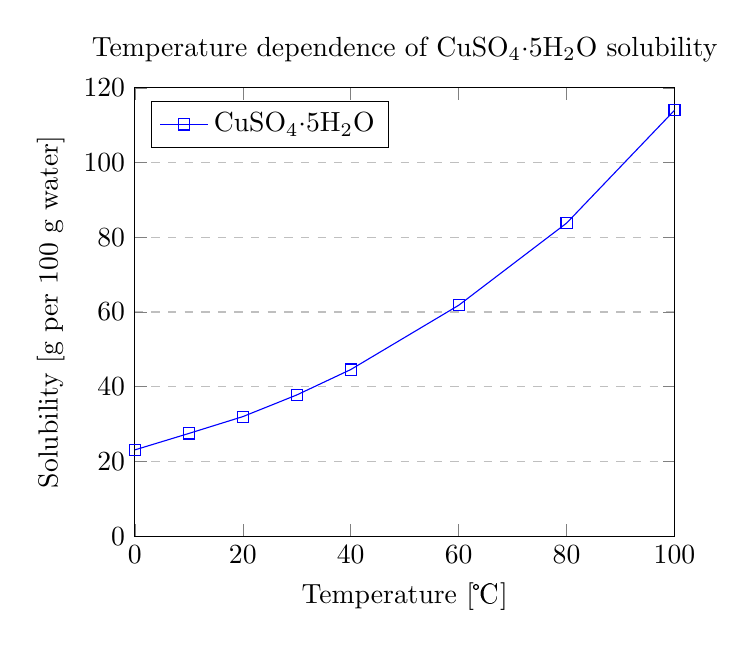
\begin{tikzpicture}
\begin{axis}[
    title={Temperature dependence of CuSO$_4\cdot$5H$_2$O solubility},
    xlabel={Temperature [\textcelsius]},
    ylabel={Solubility [g per 100 g water]},
    xmin=0, xmax=100,
    ymin=0, ymax=120,
    xtick={0,20,40,60,80,100},
    ytick={0,20,40,60,80,100,120},
    legend pos=north west,
    ymajorgrids=true,
    grid style=dashed,
]
 
\addplot[
    color=blue,
    mark=square,
    ]
    coordinates {
    (0,23.1)(10,27.5)(20,32)(30,37.8)(40,44.6)(60,61.8)(80,83.8)(100,114)
    };
    \legend{CuSO$_4\cdot$5H$_2$O}
 
\end{axis}
\end{tikzpicture}
	
	
	

	
\end{document}